\newpage
\section{User}


\begin{figure}[ht]
	\centering
  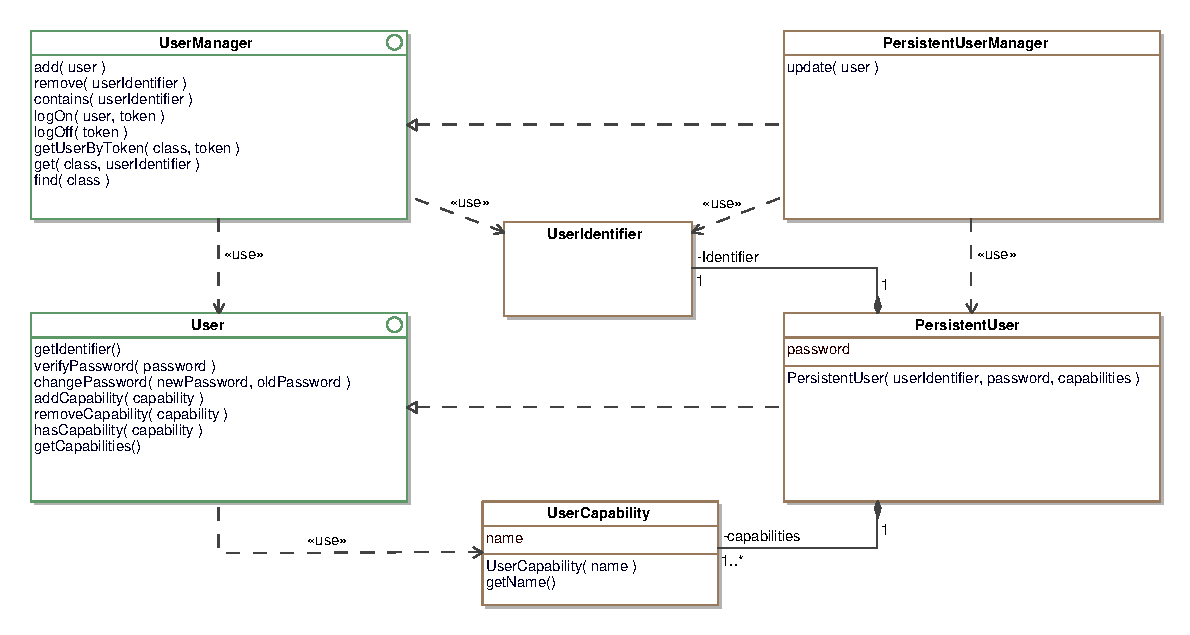
\includegraphics[width=1.0\textwidth]{images/User_Overview.eps}
	\label{user_overview}
	\caption{User - Class Overview}
\end{figure}

For implementing against interfaces we provide two in the userpackage: the \code{User} and the \code{UserManager}. The given implementions of the interfaces 
are the \code {PersistentUser} and the \code{PersistentenUserManger}. Also those two classes already provide storing \code{User}s in the database.
A \code{User} is identified by one \code{UserIdentifier} and has multiple \code{UserCapability}.


\subsection{How does it work?}

In the Salespointframework there is one \code{PersistentUsermanger}, but it is not a singleton. You can instantiate a new \code{PersistentUsermanger} whenever you need it and it always manages the same data.
The \code{UserManger} is the main part of the \code{user}-package.
You can add and remove users to/from the system.


\subsection{Ensure correct data}
To ensure having the correct data in your system you should only access users via the \code{PersistentUsermanger}:

During the process of adding a user to the system the \code{PersistentUsermanger} ensures that there will be no duplicate users. If you try to add a \code{User} with an \code{UserIdentifier} that is already in the system a \code{DuplicateUserException} will be thrown. This will help you to identify \code{Users} correctly, e.g. during the login process.

\subsection{UserCapability}
The \code{UserCapability} is a the point that helps you managing the accesses of your \code{users} in the different sections, e.g. an administrator area. Most times you combine \code{UserCapability} with your GUI to provide the different secured sections.
The \code{UserCapability} are set directly in the user. In the \code{User} you can add, remove them and ask if a the \code{User} owns a \code
{UserCapability}.


\subsection{Login}

You log in and log off your\code{User}s in the \code{PersistenceUserManger}. Therefore you generate a token and associate the token with the \code{User} in 
\code{PersistenceUserManger}.




